\section{Reconstructing Single and Double Point Sources}
\label{s:results_main}

\subsection{Input}
\label{s:results_input}
\paragraph{}We have considered the images of single point source with illumination 
at center pixel of the image and double point sources with at centre
and along the main diagonal. Both point sources have different fluxes and 
ratio of the fluxes at center to other is 0.8. We have used following input parameters
for the algorithms. 

\subsection{Input Parameters}
\label{s:results_input_p}
\paragraph{} Following are the input parameters used for reconstruction. 
\begin{itemize}
 \item Lipschitz constant ($L$) (for fixed step size variants) = maximum eigenvalue of $A^\dagger A$.
 \item Backtracking parameter ($\eta$) = 1.125.
 \item Varied Penalty parameter from ($10^{-4} < \lambda < 10^4$).
 \item Maximum Iteration Number ($maxiter$) = 10000.
 \item Tolerance limit = $10^{-7}$.
\end{itemize}

\subsection{Output}
\label{s:results_output}

\paragraph{}Figure \ref{Figsps} with $\lambda=1150$ shows reconstructed image of single point source of flux 0.4 at the center.
We had produced such images for various values of $\lambda$ to check the effect of $\lambda$ on
reconstruction. 

\paragraph{}Figure \ref{Figdps} with $\lambda=1150$ shows reconstructed image of double point source at specific
pixels. Recovered image has to ratio of fluxes (flux at center pixel : flux at other) is $\sim$ 0.8.

\begin{figure}[!htbp]
  \begin{center}
      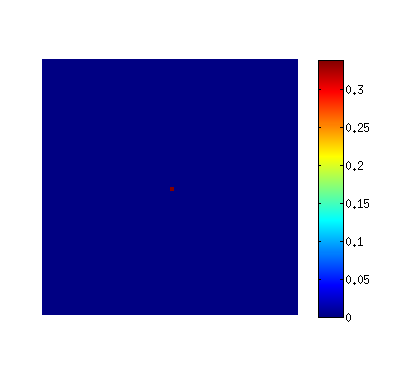
\includegraphics[width=5in,height=4in]{figures/sps}
    \caption{Reconstructed Image of Single point source with $\lambda$ = 1150}
    \label{Figsps}
  \end{center}
\end{figure}

\begin{figure}[!htbp]
  \begin{center}
      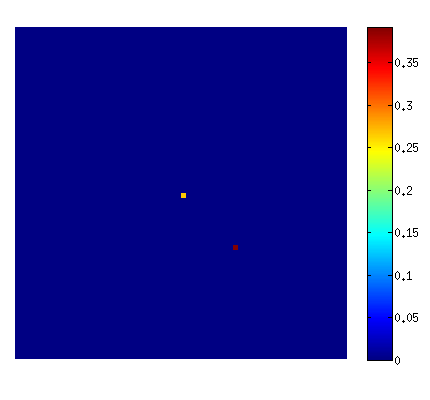
\includegraphics[width=5in,height=4in]{figures/dps}
    \caption{Reconstructed Image of Double point source with $\lambda$ = 1150}
    \label{Figdps}
  \end{center}
\end{figure}

\paragraph{}Figure \ref{Figsubplot} shows the reconstructed image with different
$\lambda$ values for all solvers. $Fista_F$ denotes Fista with fixed step size and 
similarly others.

\begin{figure}[!htbp]
  \begin{center}
      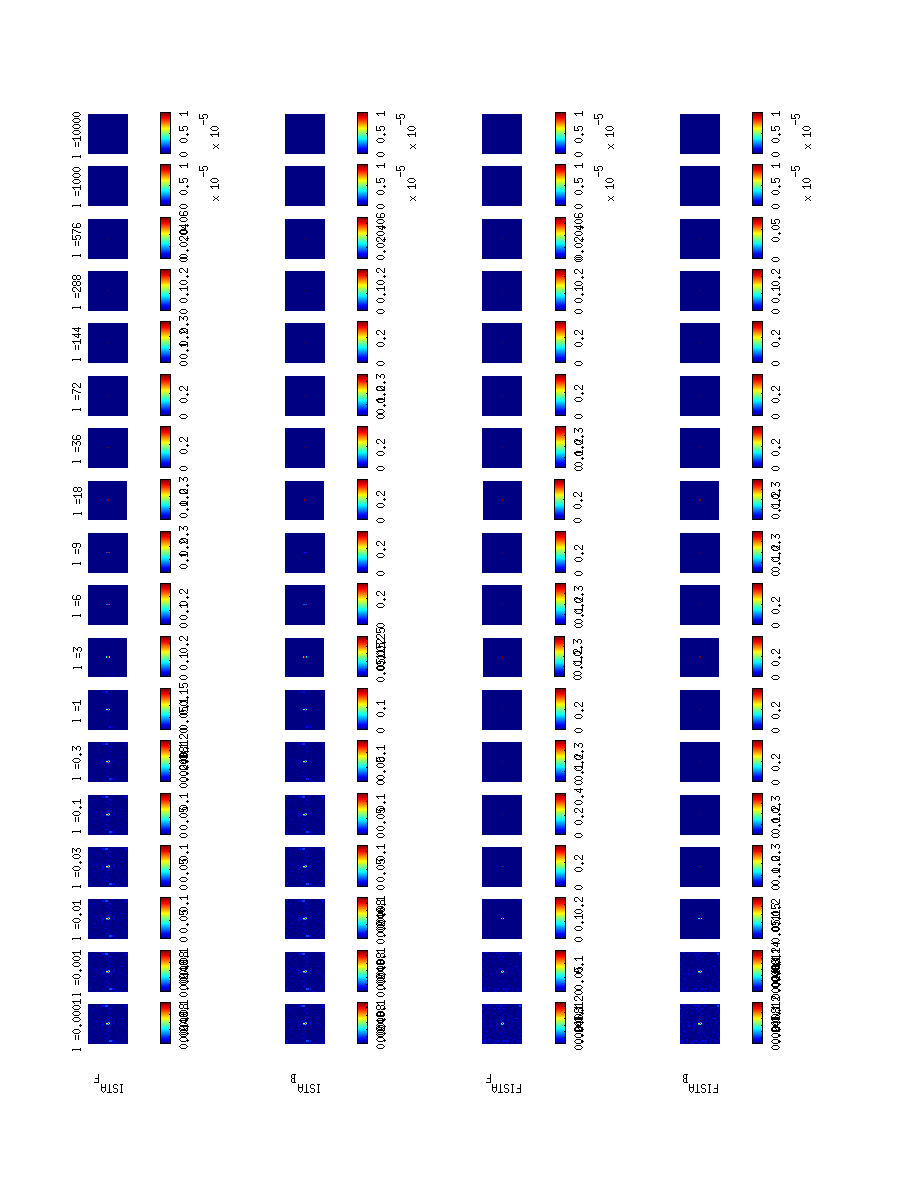
\includegraphics[width=7in,height=8in]{figures/subplots}
    \caption{Reconstructed Image of Double point source with $\lambda$ = 1150}
    \label{Figsubplot}
  \end{center}
\end{figure}
